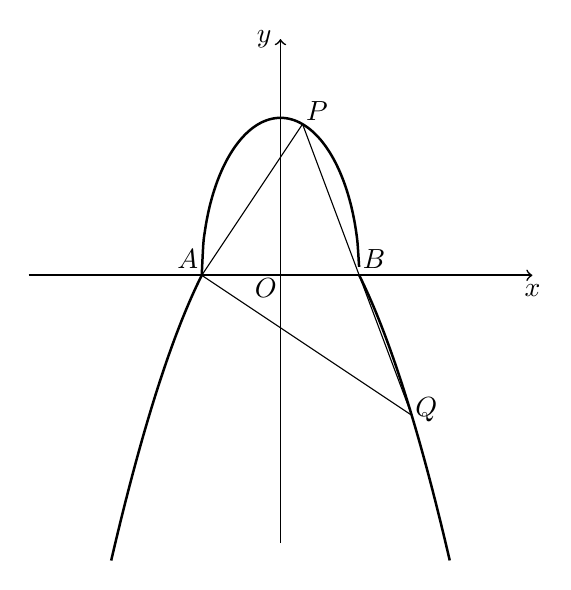
\begin{tikzpicture}[x=1cm,y=1cm,line width=0.6pt]
  \draw[black,->] (-3.2,0) -- (3.2,0);
  \node[inner sep=1pt,font=\normalsize,below,xshift=0.00bp,yshift=-2.00bp] at (3.2,0) {$x$};
  \draw[black,->] (0,-3.4) -- (0,3.0);
  \node[inner sep=1pt,font=\normalsize,left,xshift=-2.00bp,yshift=0.00bp] at (0,3.0) {$y$};
  \node[inner sep=1pt,font=\normalsize,below left] at (0,0) {$O$};
  % upper half ellipse C1: y = 2*sqrt(1-x^2), |x|<=1, thick
  \draw[black,line width=0.9pt,domain=-1:1,samples=100,smooth,variable=\x] plot ({\x},{2*sqrt(1-\x*\x)});
  % lower parabola C2: y = 1-x^2 for |x|>=1 (y<=0), thick
  \draw[black,line width=0.9pt,domain=-2.15:-1,samples=60,smooth,variable=\x] plot ({\x},{1-\x*\x});
  \draw[black,line width=0.9pt,domain=1:2.15,samples=60,smooth,variable=\x] plot ({\x},{1-\x*\x});
  % points on line l through B with slope -8/3
  \coordinate (A) at (-1,0);
  \coordinate (B) at (1,0);
  \coordinate (P) at (0.28,1.92);
  \coordinate (Q) at (1.666666667,-1.777777778);
  % segments: A-P, P-B (part of l), B-Q (part of l), A-Q
  \draw[black,thin] (A) -- (P);
  \draw[black,thin] (P) -- (Q);
  \draw[black,thin] (A) -- (Q);
  \node[inner sep=1pt,font=\normalsize,left,xshift=0.00bp,yshift=6.00bp] at (-1,0) {$A$};
  \node[inner sep=1pt,font=\normalsize,right,xshift=0.00bp,yshift=6.00bp] at (1,0) {$B$};
  \node[inner sep=1pt,font=\normalsize,above right] at (0.28,1.92) {$P$};
  \node[inner sep=1pt,font=\normalsize,right,xshift=0.00bp,yshift=2.00bp] at (Q) {$Q$};
\end{tikzpicture}
